\documentclass[tikz,border=6pt]{standalone}
% Shared figure style for the Space Data Network whitepapers.
\usepackage{lmodern}
\usepackage[T1]{fontenc}
\usepackage{xcolor}
\usetikzlibrary{arrows.meta,positioning,calc,fit,backgrounds,matrix}
\hyphenpenalty=10000\exhyphenpenalty=10000
\definecolor{ink}{HTML}{1F2328}
\definecolor{rule}{HTML}{57606A}
\definecolor{panel}{HTML}{F3F4F6}
\definecolor{accent}{HTML}{D4880F}
\tikzset{
  every picture/.style={line width=0.6pt, draw=ink, text=ink, font=\small},
  box/.style={draw=ink, fill=panel, rounded corners=2pt, align=center, inner sep=5pt},
  plain/.style={draw=ink, fill=white, rounded corners=2pt, align=center, inner sep=5pt},
  title/.style={font=\bfseries\small},
  where/.style={font=\scriptsize\itshape, text=rule},
  note/.style={font=\footnotesize\itshape, text=rule},
  flow/.style={-{Stealth[length=2.2mm]}, draw=rule},
}

\begin{document}
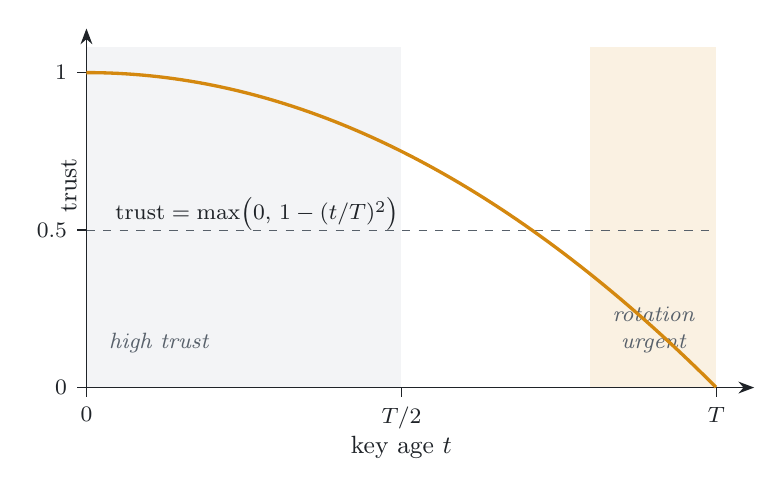
\begin{tikzpicture}[x=80mm, y=40mm]
\fill[panel] (0,0) rectangle (0.5,1.08);
\fill[accent!12] (0.8,0) rectangle (1,1.08);
\node[note, anchor=south west] at (0.02,0.08) {high trust};
\node[note, anchor=south, align=center] at (0.9,0.08) {rotation\\urgent};
\draw[rule, dashed, line width=0.3pt] (0,0.5) -- (1,0.5);
\draw[-{Stealth[length=2mm]}] (0,0) -- (1.06,0);
\draw[-{Stealth[length=2mm]}] (0,0) -- (0,1.14);
\node[below=14pt, font=\small] at (0.5,0) {key age $t$};
\node[rotate=90, above=16pt, font=\small] at (0,0.5) {trust};
\draw (0,0) -- (0,-0.03) node[below, font=\footnotesize] {$0$};
\draw (0.5,0) -- (0.5,-0.03) node[below, font=\footnotesize] {$T/2$};
\draw (1,0) -- (1,-0.03) node[below, font=\footnotesize] {$T$};
\foreach \y in {0, 0.5, 1} \draw (0,\y) -- (-0.015,\y) node[left, font=\footnotesize] {$\y$};
\draw[accent, line width=1.2pt, domain=0:1, samples=80] plot (\x, {1-\x*\x});
\node[anchor=west, font=\footnotesize] at (0.03,0.55) {$\mathrm{trust}=\max\!\left(0,\,1-(t/T)^2\right)$};
\end{tikzpicture}
\end{document}
